%%%%%%%%%%%%%%%%%%%%%%%%%%%%%%%%%%%%%%%%%
% Beamer Presentation
% LaTeX Template
% Version 1.0 (10/11/12)
%
% This template has been downloaded from:
% http://www.LaTeXTemplates.com
%
% License:
% CC BY-NC-SA 3.0 (http://creativecommons.org/licenses/by-nc-sa/3.0/)
%
%%%%%%%%%%%%%%%%%%%%%%%%%%%%%%%%%%%%%%%%%

%----------------------------------------------------------------------------------------
%	PACKAGES AND THEMES
%----------------------------------------------------------------------------------------

\documentclass{beamer}

\mode<presentation> {

% The Beamer class comes with a number of default slide themes
% which change the colors and layouts of slides. Below this is a list
% of all the themes, uncomment each in turn to see what they look like.

%\usetheme{default}
%\usetheme{AnnArbor}
%\usetheme{Antibes}
%\usetheme{Bergen}
%\usetheme{Berkeley}
%\usetheme{Berlin}
%\usetheme{Boadilla}
%\usetheme{CambridgeUS}
%\usetheme{Copenhagen}
%\usetheme{Darmstadt}
%\usetheme{Dresden}
%\usetheme{Frankfurt}
%\usetheme{Goettingen}
%\usetheme{Hannover}
%\usetheme{Ilmenau}
%\usetheme{JuanLesPins}
%\usetheme{Luebeck}
\usetheme{Madrid}
%\usetheme{Malmoe}
%\usetheme{Marburg}
%\usetheme{Montpellier}
%\usetheme{PaloAlto}
%\usetheme{Pittsburgh}
%\usetheme{Rochester}
%\usetheme{Singapore}
%\usetheme{Szeged}
%\usetheme{Warsaw}

% As well as themes, the Beamer class has a number of color themes
% for any slide theme. Uncomment each of these in turn to see how it
% changes the colors of your current slide theme.

%\usecolortheme{albatross}
%\usecolortheme{beaver}
%\usecolortheme{beetle}
%\usecolortheme{crane}
%\usecolortheme{dolphin}
%\usecolortheme{dove}
%\usecolortheme{fly}
%\usecolortheme{lily}
%\usecolortheme{orchid}
%\usecolortheme{rose}
%\usecolortheme{seagull}
%\usecolortheme{seahorse}
\usecolortheme{whale}
%\usecolortheme{wolverine}

%\setbeamertemplate{footline} % To remove the footer line in all slides uncomment this line
%\setbeamertemplate{footline}[page number] % To replace the footer line in all slides with a simple slide count uncomment this line

%\setbeamertemplate{navigation symbols}{} % To remove the navigation symbols from the bottom of all slides uncomment this line
}

\usepackage{graphicx} % Allows including images
\usepackage{booktabs} % Allows the use of \toprule, \midrule and \bottomrule in tables
\usepackage[utf8]{inputenc}
\usepackage[russian]{babel}
\usepackage{hyperref}
\usepackage{ulem}
\usepackage{amsmath}
%----------------------------------------------------------------------------------------
%	TITLE PAGE
%----------------------------------------------------------------------------------------

\title{Предсказание энергии связи} % The short title appears at the bottom of every slide, the full title is only on the title page

\author{Рак Алексей} % Your name
\date{\today} % Date, can be changed to a custom date

\begin{document}

\begin{frame}
\titlepage % Print the title page as the first slide
\end{frame}

\begin{frame}
\frametitle{План} % Table of contents slide, comment this block out to remove it
\tableofcontents % Throughout your presentation, if you choose to use \section{} and \subsection{} commands, these will automatically be printed on this slide as an overview of your presentation
\end{frame}

%----------------------------------------------------------------------------------------
%	PRESENTATION SLIDES
%----------------------------------------------------------------------------------------

%------------------------------------------------
\section{Используемые данные} % Sections can be created in order to organize your presentation into discrete blocks, all sections and subsections are automatically printed in the table of contents as an overview of the talk
%------------------------------------------------

\begin{frame}
\frametitle{Используемые данные}\begin{center}
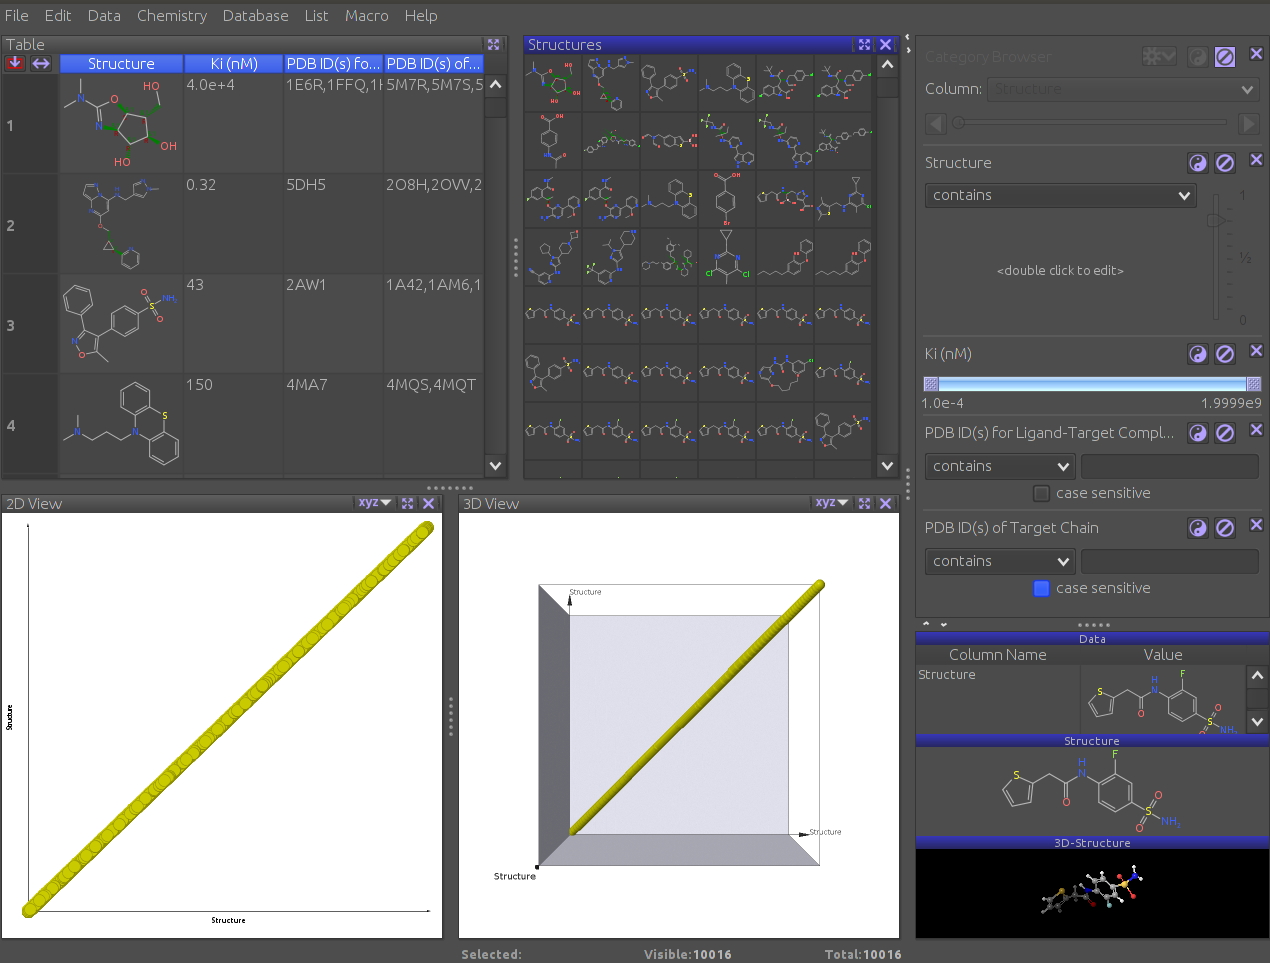
\includegraphics[scale=0.2]{used_data.png}
\end{center}
\end{frame}

\begin{frame}
\frametitle{Используемые данные}
Какие данные используются:
\begin{itemize}
\pause
\item Структура лиганда\pause
\item Ki (энергия связи)\pause
\item Id белка в pdb\pause
\item Id комлпекса в pdb\pause
\end{itemize}
\end{frame}

%------------------------------------------------
\section{Теория} % Sections can be created in order to organize your presentation into discrete blocks, all sections and subsections are automatically printed in the table of contents as an overview of the talk
%------------------------------------------------
\subsection{Нейронные Сети}
\begin{frame}
\frametitle{Нейронные сети}\begin{center}
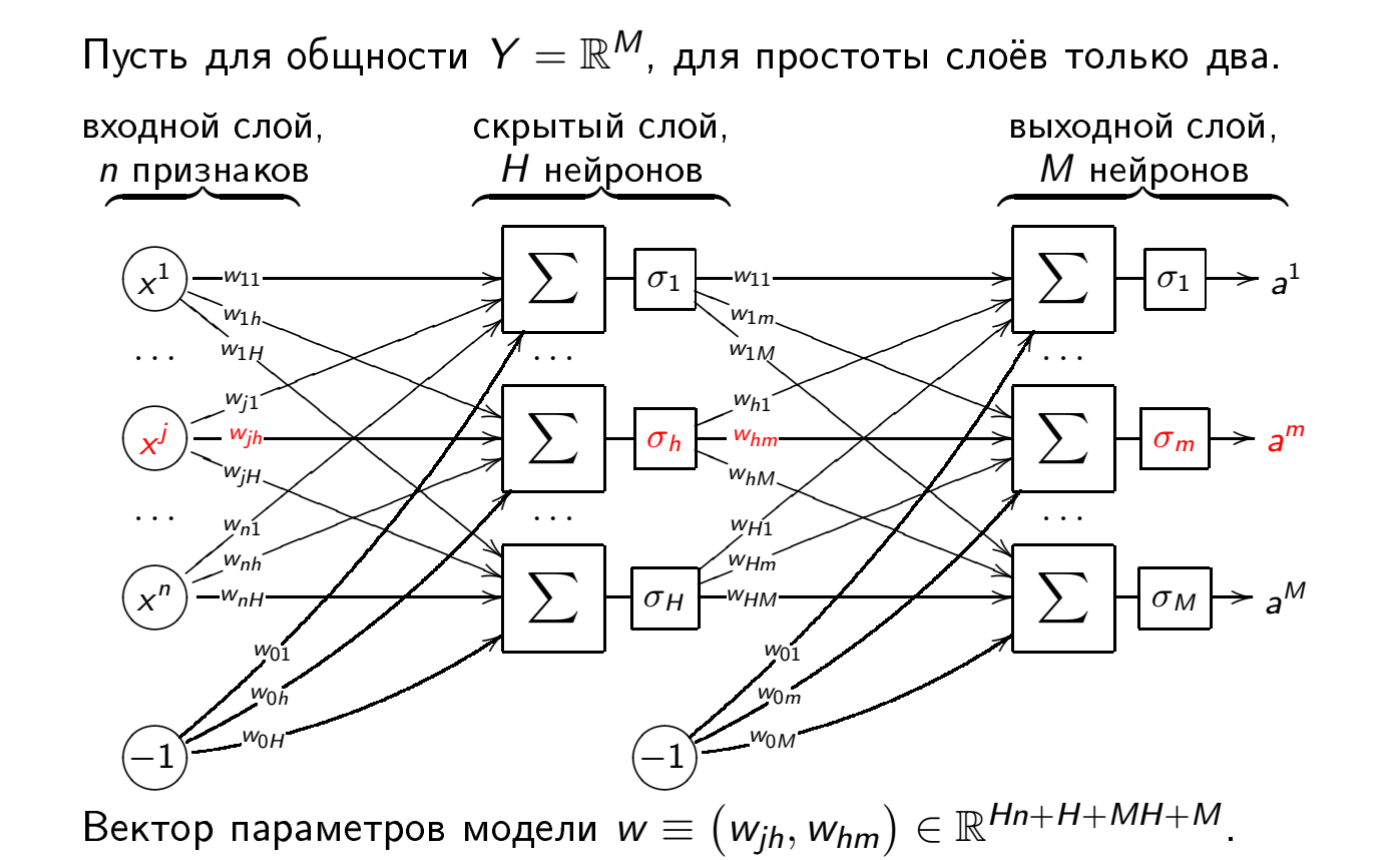
\includegraphics[scale=0.3]{neurel_network.png}
\end{center}
\end{frame}

\begin{frame}
\frametitle{Нейронные сети}
\pause
\begin{itemize}
\item Позволяют решать широкий класс задач\pause
\item Метод обратного распространения ошибки - основанный на простейшем правиле дифференцирования сложной функции, позволяет учить нейронные сети\pause
\item Очень много способов улучшать сходимость и качество нейросети:\pause
\begin{itemize}
\item Регуляризация\pause
\item Перетасовка объектов\pause
\item Разные градиентные методы\pause
\item Адаптивный learning rate\pause
\item Dropout\pause
\item Разные функции активации\pause
\item Аугментация (расширение выборки)\pause
\end{itemize}
\end{itemize}
\end{frame}

\subsection{Свёрточные нейронные сети}
\begin{frame}
\frametitle{Свёрточные нейронные сети}\begin{center}
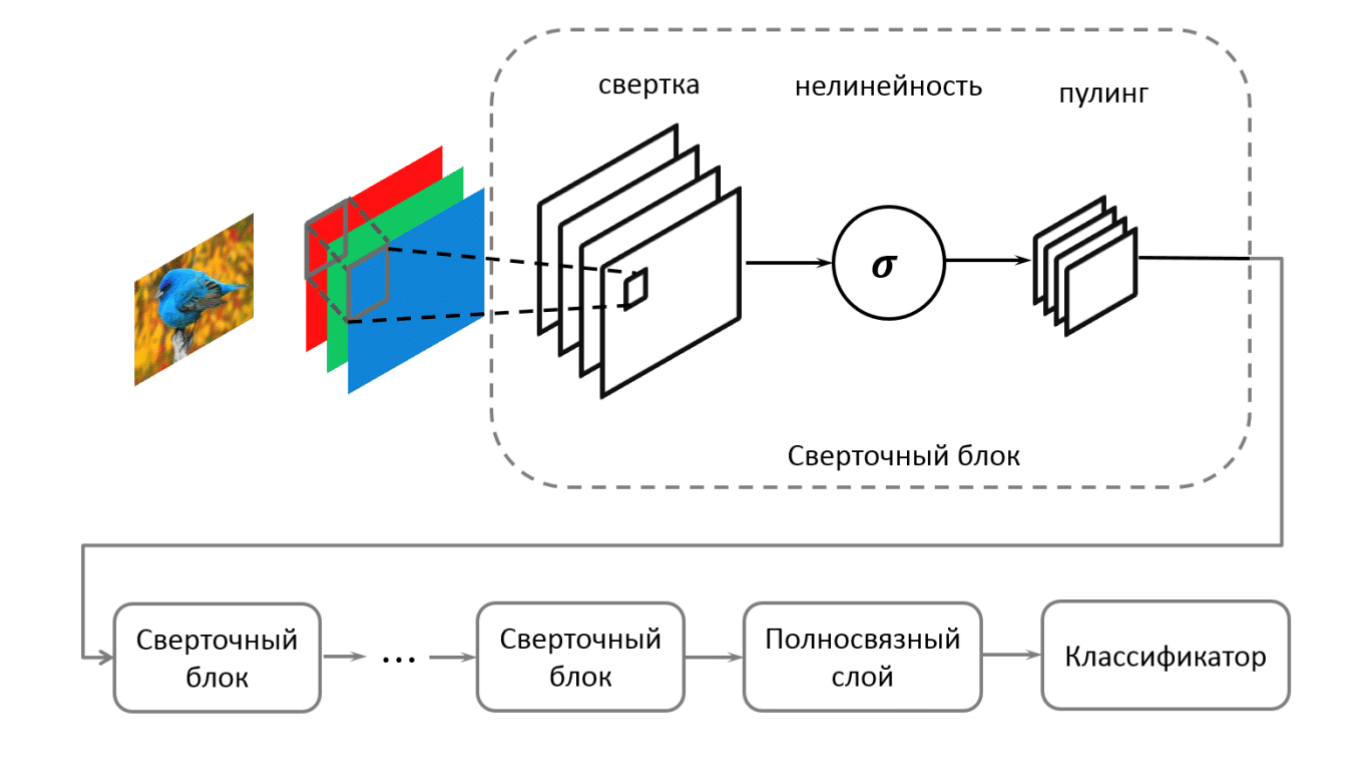
\includegraphics[scale=0.3]{convolutional_nn.png}
\end{center}
\end{frame}

\begin{frame}
\frametitle{Свёрточный слой}\begin{center}
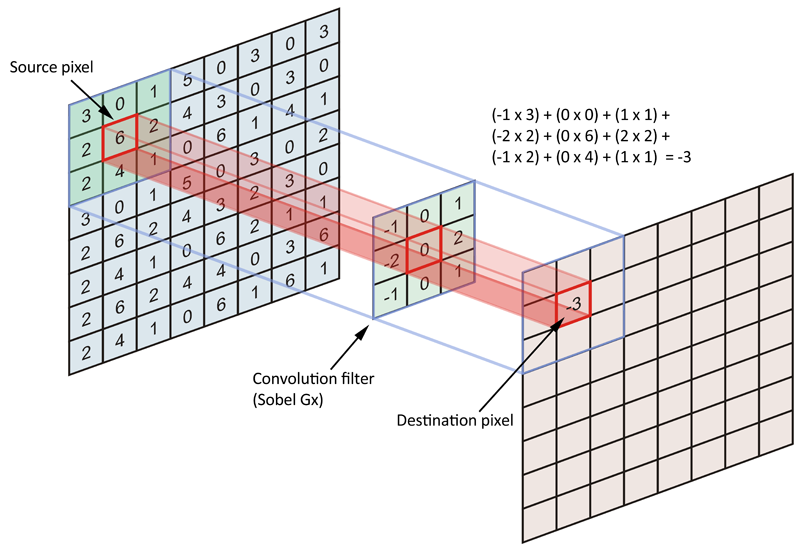
\includegraphics[scale=0.3]{convolutional_layer.png}
\end{center}
\end{frame}

\begin{frame}
\frametitle{Пулинг слой}\begin{center}
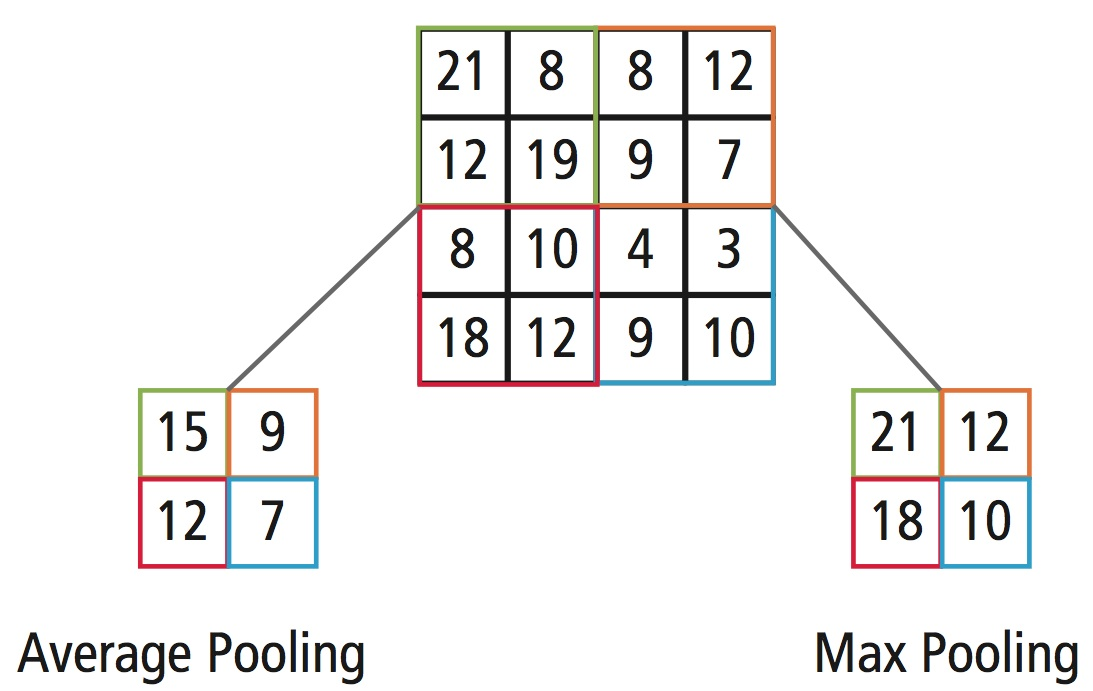
\includegraphics[scale=0.3]{pooling.jpg}
\end{center}
\end{frame}


\subsection{Атомная свёрточная сеть}
\begin{frame}
\frametitle{Атомная свёрточная сеть}\begin{center}
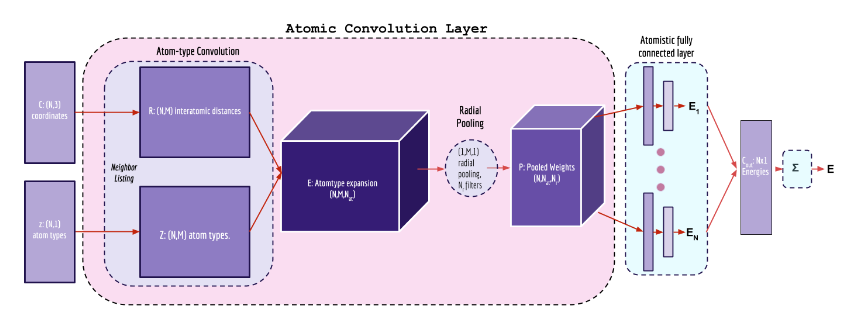
\includegraphics[scale=0.4]{atomic_convolution_nn.png}
\end{center}
\end{frame}

\begin{frame}
\frametitle{Начальное преобразование данных}
\begin{itemize}
\pause
\item На вход поступает матрица атомов, которая содерижт атомный тип каждого атома и его трёхмерные координаты.\pause
\item Преобразуем эту матрицу в 2 матрицы R и Z размера (N x M), где N -- это число атомов, M -- число рассматриваемых соседей (в работе было равно 12).
\begin{itemize}
\item R -- матрица расстояний до соседей.
\item Z -- матрица атомных типов соседей.
\end{itemize}
\end{itemize}
\end{frame}

\begin{frame}
\frametitle{Атомный свёрточный слой}
\begin{itemize}
\pause
\item На входе этого этапа мы получаем 2 матрицы две матрицы R и Z.\pause
\item $N_{at}$ -- число различных атомных типов в данных. \pause
\item $K_{ij}^a = \begin{cases} 1, Z_{i,j} = N_a\\
0, $иначе$\end{cases}$\pause
\item $(K * R)_{ij}^a = R_{ij}K_{ij}^a$\pause
\item Применив такие операции мы получаем матрицу E размера ($N$, $M$, $N_{at}$)  
\end{itemize}
\end{frame}

\begin{frame}
\frametitle{Атомный пулинговый слой}
\begin{itemize}
\pause
\item На входе этого этапа мы получаем матрицу E размера ($N$, $M$, $N_{at}$).\pause
\item $f_s (r_{ij}) = \exp{\left(-\frac{(r_{ij} - r_s)^2}{\sigma_s^2}f_c(r_{ij})\right)}$ \pause
\item $f_c (r_{ij}) = \begin{cases}\frac{1}{2}\cos{\left(\frac{\pi r_{ij}}{R_c}\right)}, 0 < r_{ij} < R_c\\
0, r_{ij} \geq R_c
\end{cases}$ \pause
\item $P_{i, n_a, n_r} = \beta_n \sum_{i = 1}^{M} f_{n_r}(E_{ijn_a}) + b_{n_r}$\pause
\item В итоге мы получаем матрицу P размера ($N$, $N_a$, $N_r$)\pause
\item $r_s, \sigma_s$ -- обучаемы параметры.\pause
\item $\beta, b$ -- постоянные выбираемые до обучения.\pause
\end{itemize}
\end{frame}

\begin{frame}
\frametitle{Атомный полносвязный слой}
\begin{itemize}
\pause
\item На входе этого этапа мы получаем матрицу E размера ($N$, $N_{at}$, $N_{r}$).\pause
\item $N_r$ -- это число различных пулинговых фильтров.\pause
\item Затем строится двухслойная нейронная сеть, одинаковая для всех атомов, и прогоняют через неё матрицу каждого атома (1, $N_{at}$, $N_r$)\pause
\item Для каждого атома получаям по скаляру, которые суммируем, это и есть ответ.
\end{itemize}
\end{frame}

\begin{frame}
\frametitle{Энергия связи}\begin{center}
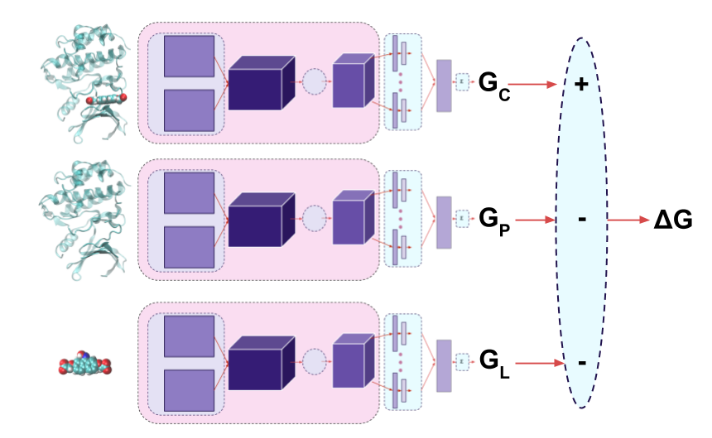
\includegraphics[scale=0.4]{energy.png}
\end{center}
\end{frame}

\begin{frame}
\frametitle{Коэффициент детерминации}
\begin{gather*}
R^2 = 1 - \frac{\hat{\sigma}^2}{\hat{\sigma_y}^2} = 1 - \frac{SS_{res} / n}{SS_{tot} / n} = 1 - \frac{SS_{res}}{SS_{tot}}\\
SS_{res} = \sum_{i = 1}^{n} (y_i - \hat{y_i})^2\\
SS_{tot} = \sum_{i=1}^{n} (y_i - \bar{y})^2\\
\bar{y} = \frac{1}{n}\sum_{i=1}^n y_i
\end{gather*}
$y_i$ --  фактическое значение, $\hat{y_i}$ -- расчётное значение
\end{frame}

\begin{frame}
\frametitle{Результаты}

\begin{center}
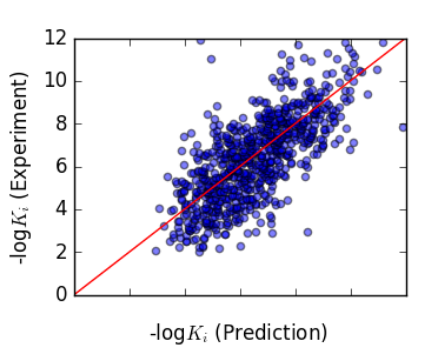
\includegraphics[scale=0.6]{res.png}
\end{center}
\end{frame}
\end{document}